\chapter*{perception}
\addcontentsline{toc}{chapter}{perception}
\begin{center}
\vspace{2cm}
\begin{flushright}
\textit{Loud drones, low frequency soothing sounds\\Whispers louder than the loudest screams\\A new detail that changed my day\\The repetitive, unsettling touch\\Tight knots, tight hugs\\Invasive gazes that were not supposed to last\\The faces, the mirrors, the shadows\\Acoustics as the language of every surface}\\
\textbf{M.V.} 
\end{flushright}
\vspace{2cm}
% \vspace*{\fill}
\end{center}
\normalsize

\newpage  % Move to the next page
Self-Organized Criticality describes how certain systems naturally evolve toward a critical, highly sensitive state where small changes can lead to large-scale effects. This state of criticality is "self-organized" because the system doesn't require external tuning to reach this point. It naturally arranges itself into this state through its own dynamics. These models help describe the experience of sensory amplification, where the world can be perceived in vivid detail or with overwhelming intensity. \citep{adami1993}

This idea resonates with my perception of sensory experiences, where seemingly minor stimuli can trigger profound shifts in awareness. My engagement with immersive media and neurophysiological responses to sensory inputs mirrors the principles of self-organized criticality, where perception can oscillate between stability and heightened sensitivity without external modulation. Just as a sandpile reaches a delicate equilibrium where a single grain can trigger a cascade, perception often reaches states where minor inputs lead to significant experiential shifts.

%% image
\begin{figure}
    \centering
    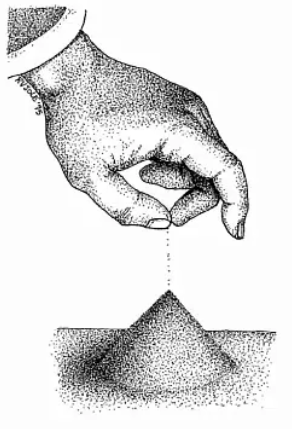
\includegraphics[width=0.8\linewidth]{assets/sandpile.png} 
    \caption{\small Self organized criticality - \textit{Per Bak's Sand pile model, 1988}.}
    \label{fig:sandpile}
\end{figure}

For many, perception unfolds in ways that might differ from conventional understandings. It is often nonlinear and multisensorial, difficult to articulate but deeply felt. The context and balances between anxiety and relaxation shape the sensitivity to sounds and textures. Patterns and structures in an otherwise chaotic environment can be a comforting experience. Time feels non-linear, with moments stretching or compressing, influencing how art and events are experienced.

Immersive or interactive art forms, such as installation art, allow for the direct engagement of multiple senses, mirroring how individuals process the world, translating complex inner experiences into tangible forms. Sensory overload or hyperfocus can transform the relationship between body and world, defining new ways to conceptualize subjectivity.

From a physics standpoint, perception can be understood as a signal processing system, where sensory organs act as transducers, converting energy from one form to another. Interacting photons, wavelengths of a restricted spectrum, pressure variations converted into electrical signals, molecules binding and interacting with receptors, mechanical interactions of skin cells, electromagnetic repulsion, preventing matter from collapsing into itself.

Physics reveals that human perception captures only a small fraction of reality. Neutrinos, dark matter, infrared and ultraviolet light, gravitational waves, and radio signals are imperceptible to us, but part of this reality can be detected with specialized instruments. Can the use of such instruments alter our perception? Is it possible to amplify and alter the ways we relate to the environment by increasing the reach of our perception?

Technology expands our Umwelt by allowing us to access phenomena that are otherwise absent from our perceptual sphere. From infrared imaging to quantum computers, from microscopes to large language models, technology acts as an extension of our perceptual apparatus, expanding our boundaries into previously inaccessible domains.

However, expanding the Umwelt through technological augmentation also transforms the sensorium, the historically contingent ways in which cultures structure perception. Friedrich Kittler and other media theorists have emphasized that new media do not merely extend human perception, but create entirely new perceptual regimes, where what is seen, heard, and felt is structured by technical systems. As Kittler observes in Optical Media (Berlin Lectures, 1999), "\textit{Media determine our situation. If the optical nerve is replaced by fiber-optic cables, then perception itself is no longer an autonomous act but a function of transmission speeds.}"\citep{kittler1999}. This suggests that contemporary digital infrastructures, ranging from algorithmic filtering to surveillance systems and AI-driven vision, do not merely mediate perception but actively reshape what is perceptible and how sensory data is processed.

% note: examples for previous paragraph 

The field of sensorium studies explores how haptic, auditory, and visual perception are mediated through evolving interfaces, from VR and haptics to biometric sensors. In this context, the question is not just about accessing new perceptual domains but about who controls the mediation of those domains. If perception is increasingly outsourced to technological systems, how does this alter the relationship between self, body, and world?


According to the philosophical approach of post-phenomenology, technology is not neutral. It transforms the nature of perception and experience. Instruments shape what and how we perceive, influencing the object of perception as well as the perceiver.

Our brain is remarkably adaptable and capable of incorporating non-biological sensors into its perceptual framework. This phenomenon is supported by research in neuroscience, cognitive science, and philosophy, particularly in the domains of neuroplasticity, sensory substitution, and embodied cognition. The inclusion of non-biological sensors introduces entirely new dimensions to human perception, effectively expanding the "self."

The extended mind hypothesis, proposed by the philosophers Andy Clark and David Chalmers, argues that tools and technologies can become integral parts of our cognitive processes. Non-biological sensors present in wearable technologies provide continuous streams of data, which the brain learns to process and integrate. This suggests that perception is not confined to the brain and body but extends into the tools we use, fundamentally altering our experience.

While the extended mind hypothesis positions cognition as distributed beyond the brain, it has been critiqued for an overly functionalist approach that abstracts the role of media, institutions, and historical structures in shaping cognitive processes. N. Katherine Hayles, in "\textit{Unthought: The Power of the Cognitive Nonconscious}, abandons the assumption that cognition is always rational, conscious, and computationally extendable. Hayles' concept of the unthought" (the aspects of cognition that exceed conscious awareness) offers a new lens for rethinking perception beyond intentionality. She moves the discussion from what we perceive to how our cognitive frameworks themselves are shaped by technology. In her book, Hayles engages with Bernard Stiegler's theories to discuss how technological mediation affects cognitive processes, particularly in the context of automated perception and algorithmic attention capture.

In this framework, perception is not just a personal or biological act but is conditioned by material and symbolic systems that shape what can be thought or perceived. Digital and algorithmic systems increasingly mediate our experience, shifting cognitive agency away from the individual toward nonconscious, networked processes. The \textit{unthought} implies that perceptual extension via technology is not merely an augmentation but also a restructuring that operates beyond intentional human control. Hayles critically questions not just what we perceive with technology but who or what determines the structures that govern perception itself.

If perception relies on external tools, the distinction between "human" and "machine" becomes less clear, leading to a hybridized (cyborg) perception that transcends biology. What counts as "real" if our tools mediate all new experiences? Can the brain adapt to perceive entirely artificial data streams, such as simulations or virtual realities, as seamlessly as it does natural environments?  

Neural implants such as the Cochlear implant, or existing research in sensory substitution, demonstrate that artificial stimuli can be integrated into perception seamlessly, despite being electrically generated rather than naturally occurring. Experiments in VR adaptation (e.g., the rubber hand illusion, full-body swaps) indicate that the brain can incorporate entirely artificial spatial and sensory information into its embodied schema. AI, predictive algorithms, and immersive XR environments are already generating stimuli that are neurologically indistinguishable from non-mediated experience. Perception is no longer confined to biological limits but is an open system shaped by neural plasticity and technological augmentation. The notion of "reality" becomes an emergent cybernetic construct, not fixed, but fluid, shifting as cognitive architectures evolve. In this sense, the "real" is whatever perception successfully integrates, whether natural or synthetic. It becomes a category of phenomenological stability rather than an intrinsic property of the world. 

"\textit{By reenvisioning cognition and crafting a framework in which nonconscious cognition plays a prominent role, my approach enables analyses of cognitive assemblages, and the mediators operating within them, as the means by which power is created, extended, modified, and exercised in technologically developed societies.}"\citep{hayles2017}

If technological mediation fundamentally shapes perception, then perception itself becomes a site of power, where control over sensory experience is increasingly delegated to infrastructures beyond individual agency. Stiegler warns that in an era of automated perception and algorithmic attention capture, the process of individuation (the capacity to form unique sensory and cognitive patterns) is under threat. Similarly, Hayles' work on the nonconscious cognitive domain suggests that much of what we assume to be autonomous perception is pre-structured by the digital environments we inhabit. 

This calls for a critical approach to perception that does not merely celebrate augmentation but interrogates who or what is shaping perceptual thresholds. Can artistic interventions, speculative design, and critical media practices expose the hidden architectures of technological perception? And if so, how can we reclaim perceptual agency in an era of increasing sensory automation and resist the passive absorption of algorithmically curated experiences? If algorithmic perception operates by optimizing and automating attention, then one form of resistance is to introduce perceptual friction, forcing slow, deep engagement rather than passive consumption. Building alternative, decentralized, open-source tools for AI-assisted art, collective sensory experiences, and participatory XR environments might offer new spaces for perceptual experimentation outside corporate frameworks.

At the same time, the question of how we manage and regulate sensory input becomes increasingly urgent. As perception expands beyond biological limitations through technological augmentation, we are also faced with the challenge of navigating not just the enhancement but the overload of sensory information. If perception is shaped by external tools, what strategies can be developed to mitigate overstimulation while maintaining agency over sensory experience?

An overwhelming visual stimulation can sometimes be managed via a calming sound or a specific type of pressure. Since the world is evolving into larger and larger amounts of information and stimuli, it's interesting to wonder if the inclusion of new types of non-biological sensors in our perception will provoke further overstimulation or present opportunities for relaxation based on new calming sensations. Perhaps soon, focusing on calming fluctuations of cosmic microwave background radiation will provide a mental shelter from saturated visual and acoustic inputs in our present environment.


% note: maybe some examples of work that highlight this specious nature of perception, understanding and the posibility for a critique. e.g. Ikeda's installations? 


